\chapter{Results}
\section {Waveform Morphology}
\begin{figure}[H]
  \centering
    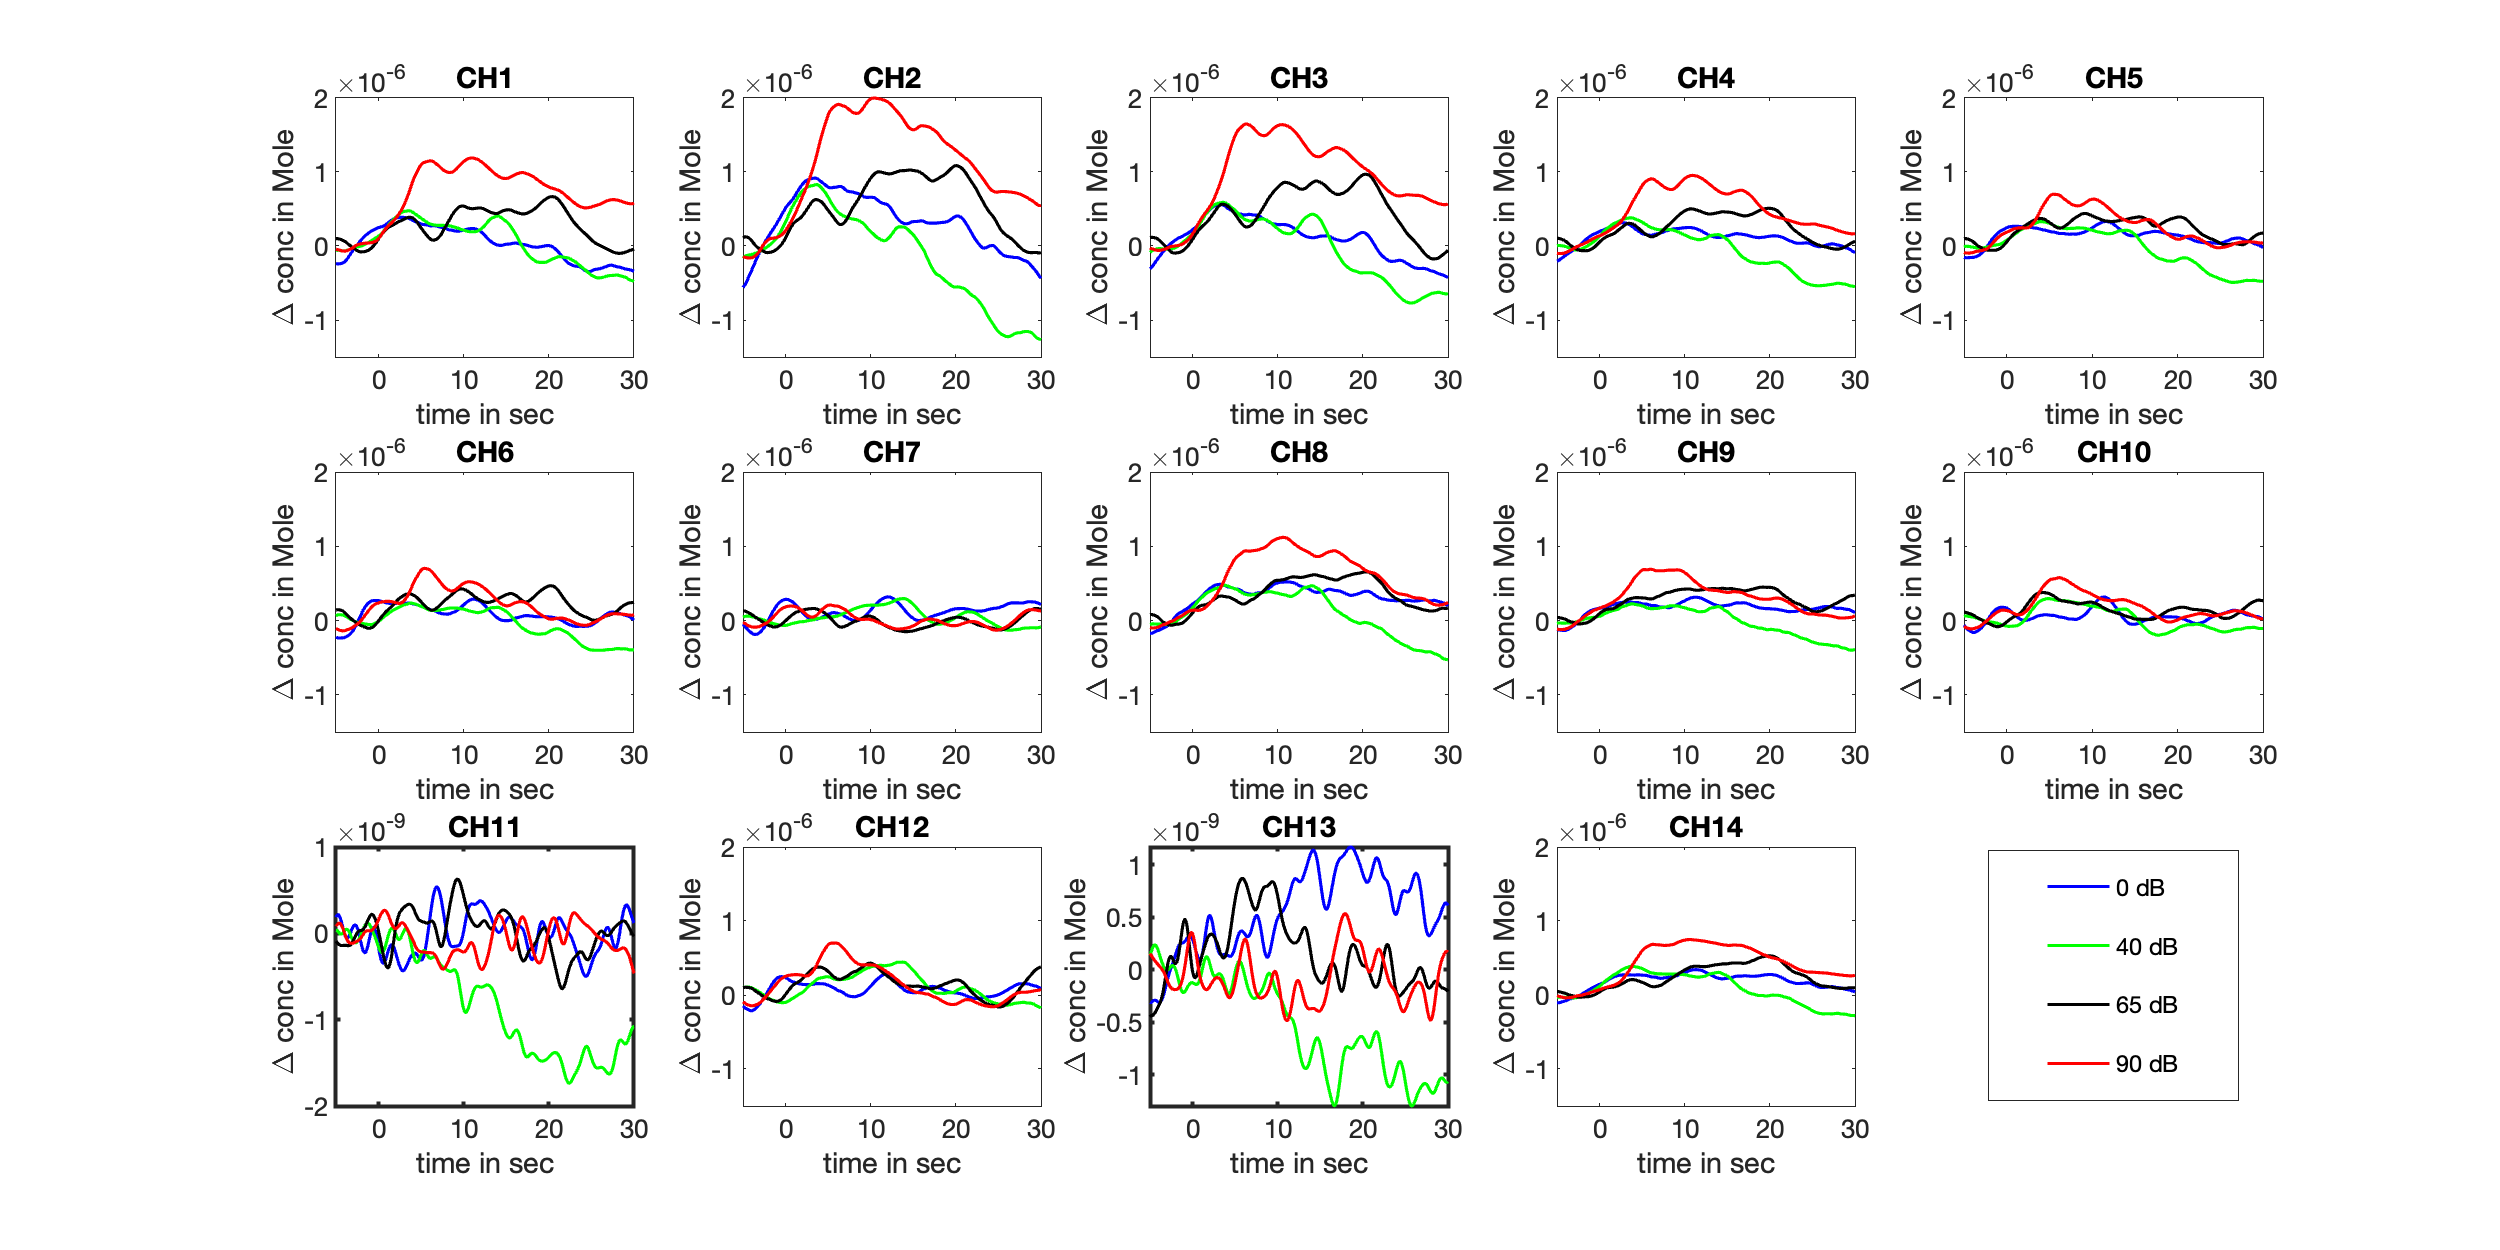
\includegraphics[scale=.4]{bilder/HbO_Mole/sub_jonas_s_HbO.png}
  \caption{Probe design in this research. Shown in AtlasViewer}
  \label{fig:somesignal}
\end{figure}

\begin{figure}[H]
  \centering
    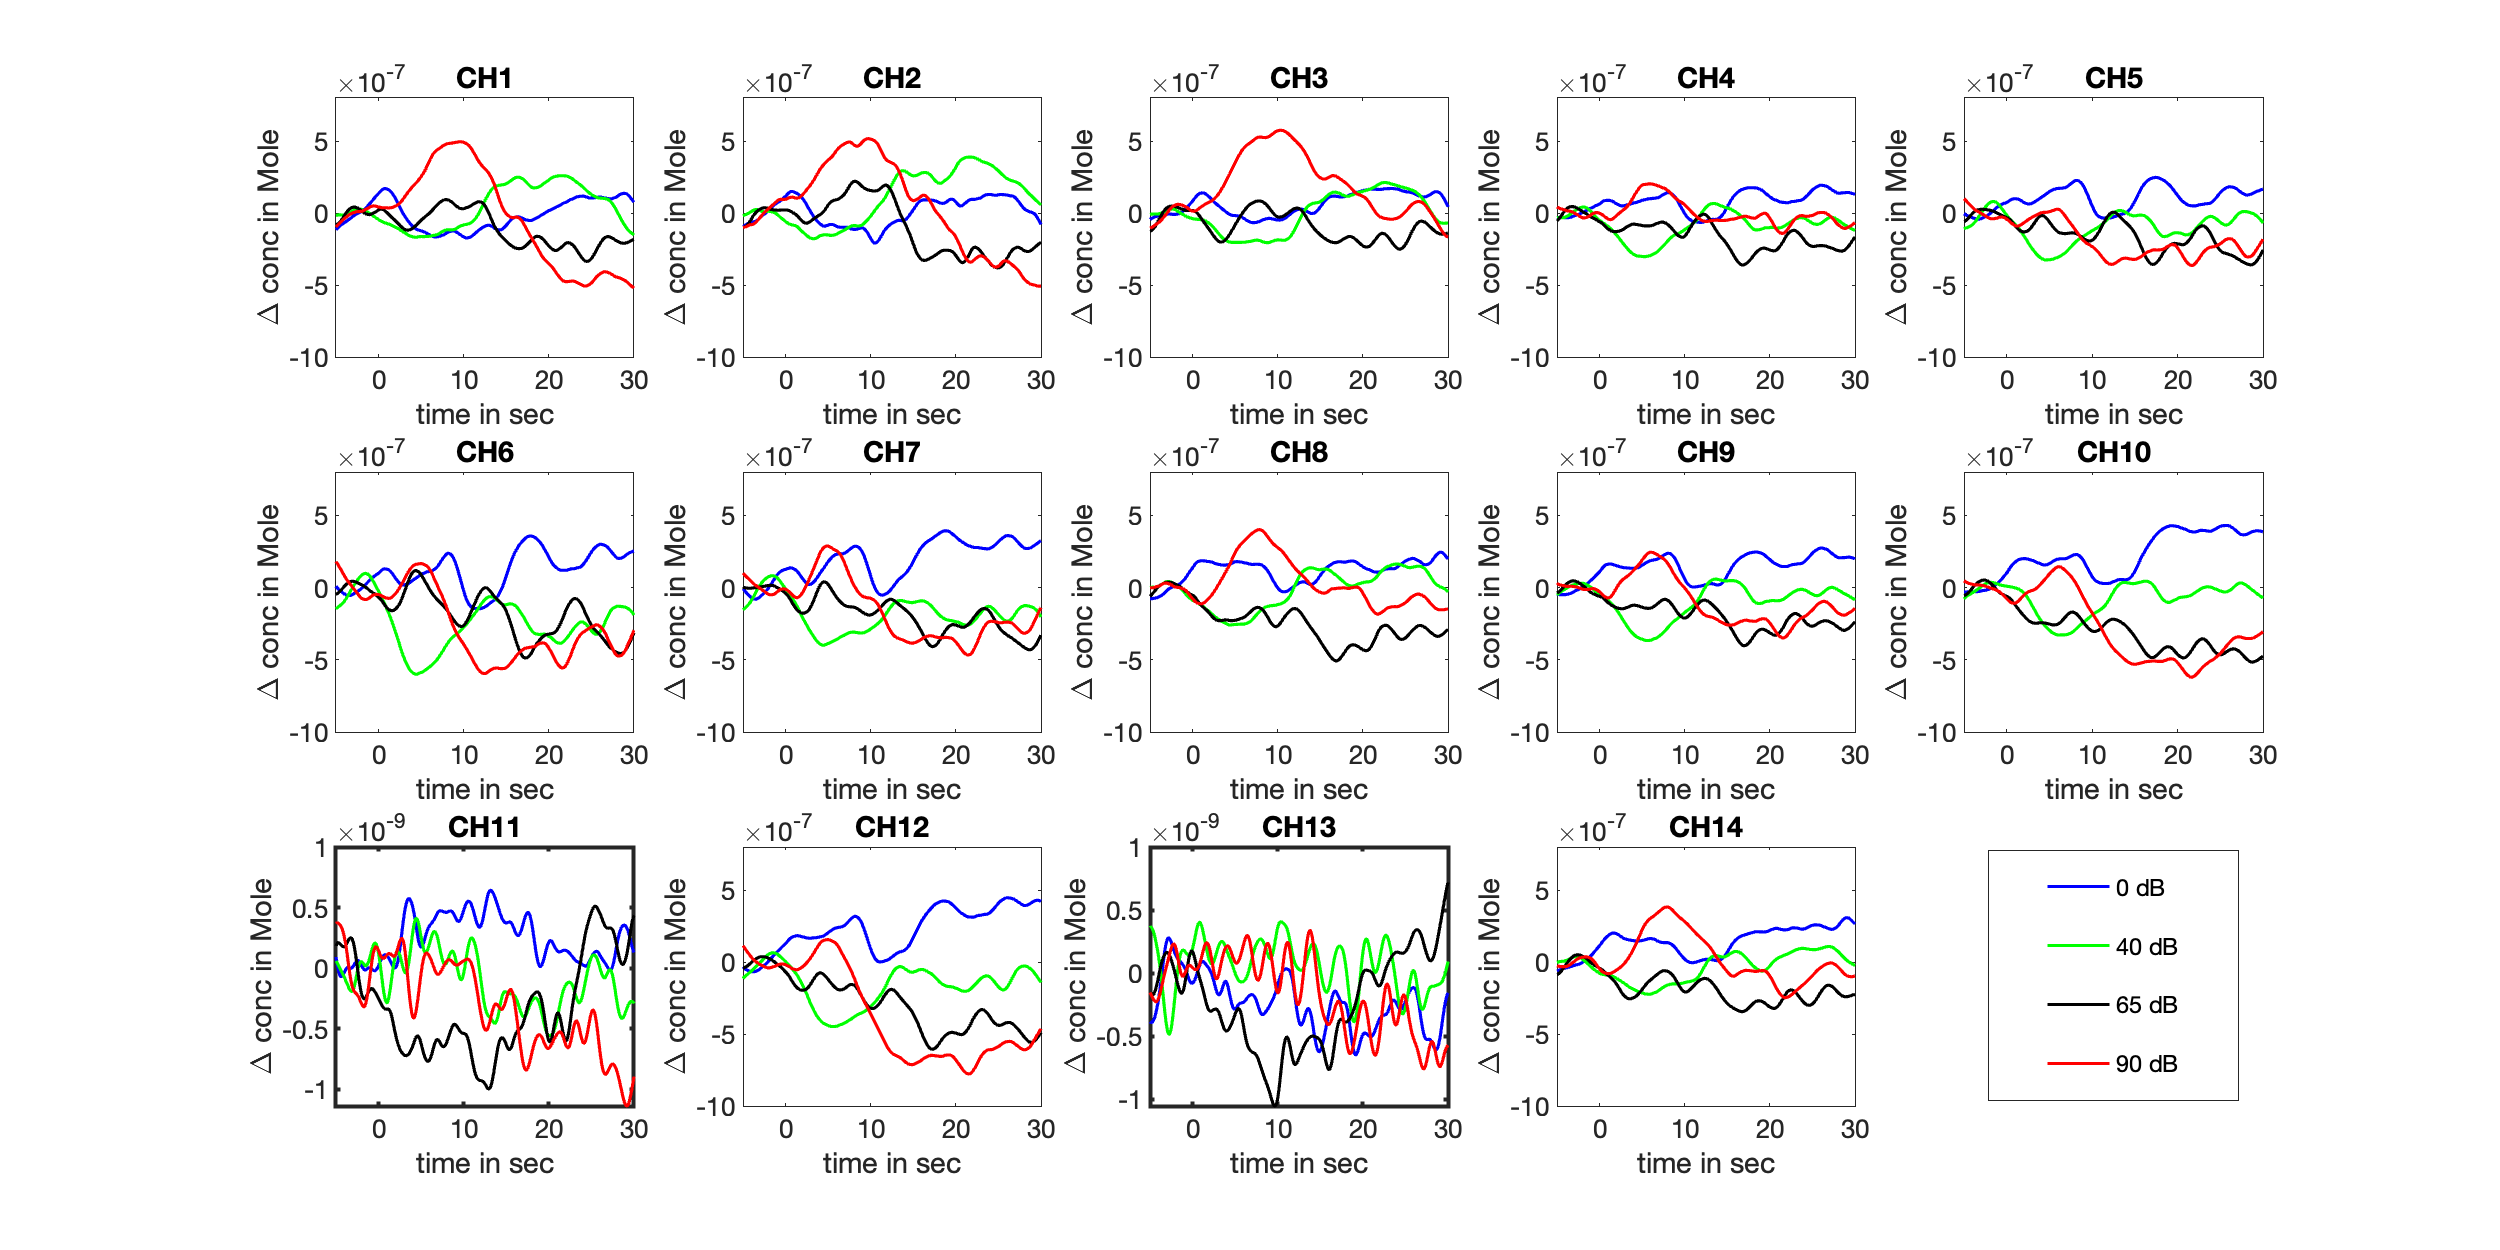
\includegraphics[scale=.4]{bilder/HbO_Mole/sub_lukas_s_HbO.png}
  \caption{Probe design in this research. Shown in AtlasViewer}
  \label{fig:somesignal}
\end{figure}


\begin{figure}[H]
  \centering
    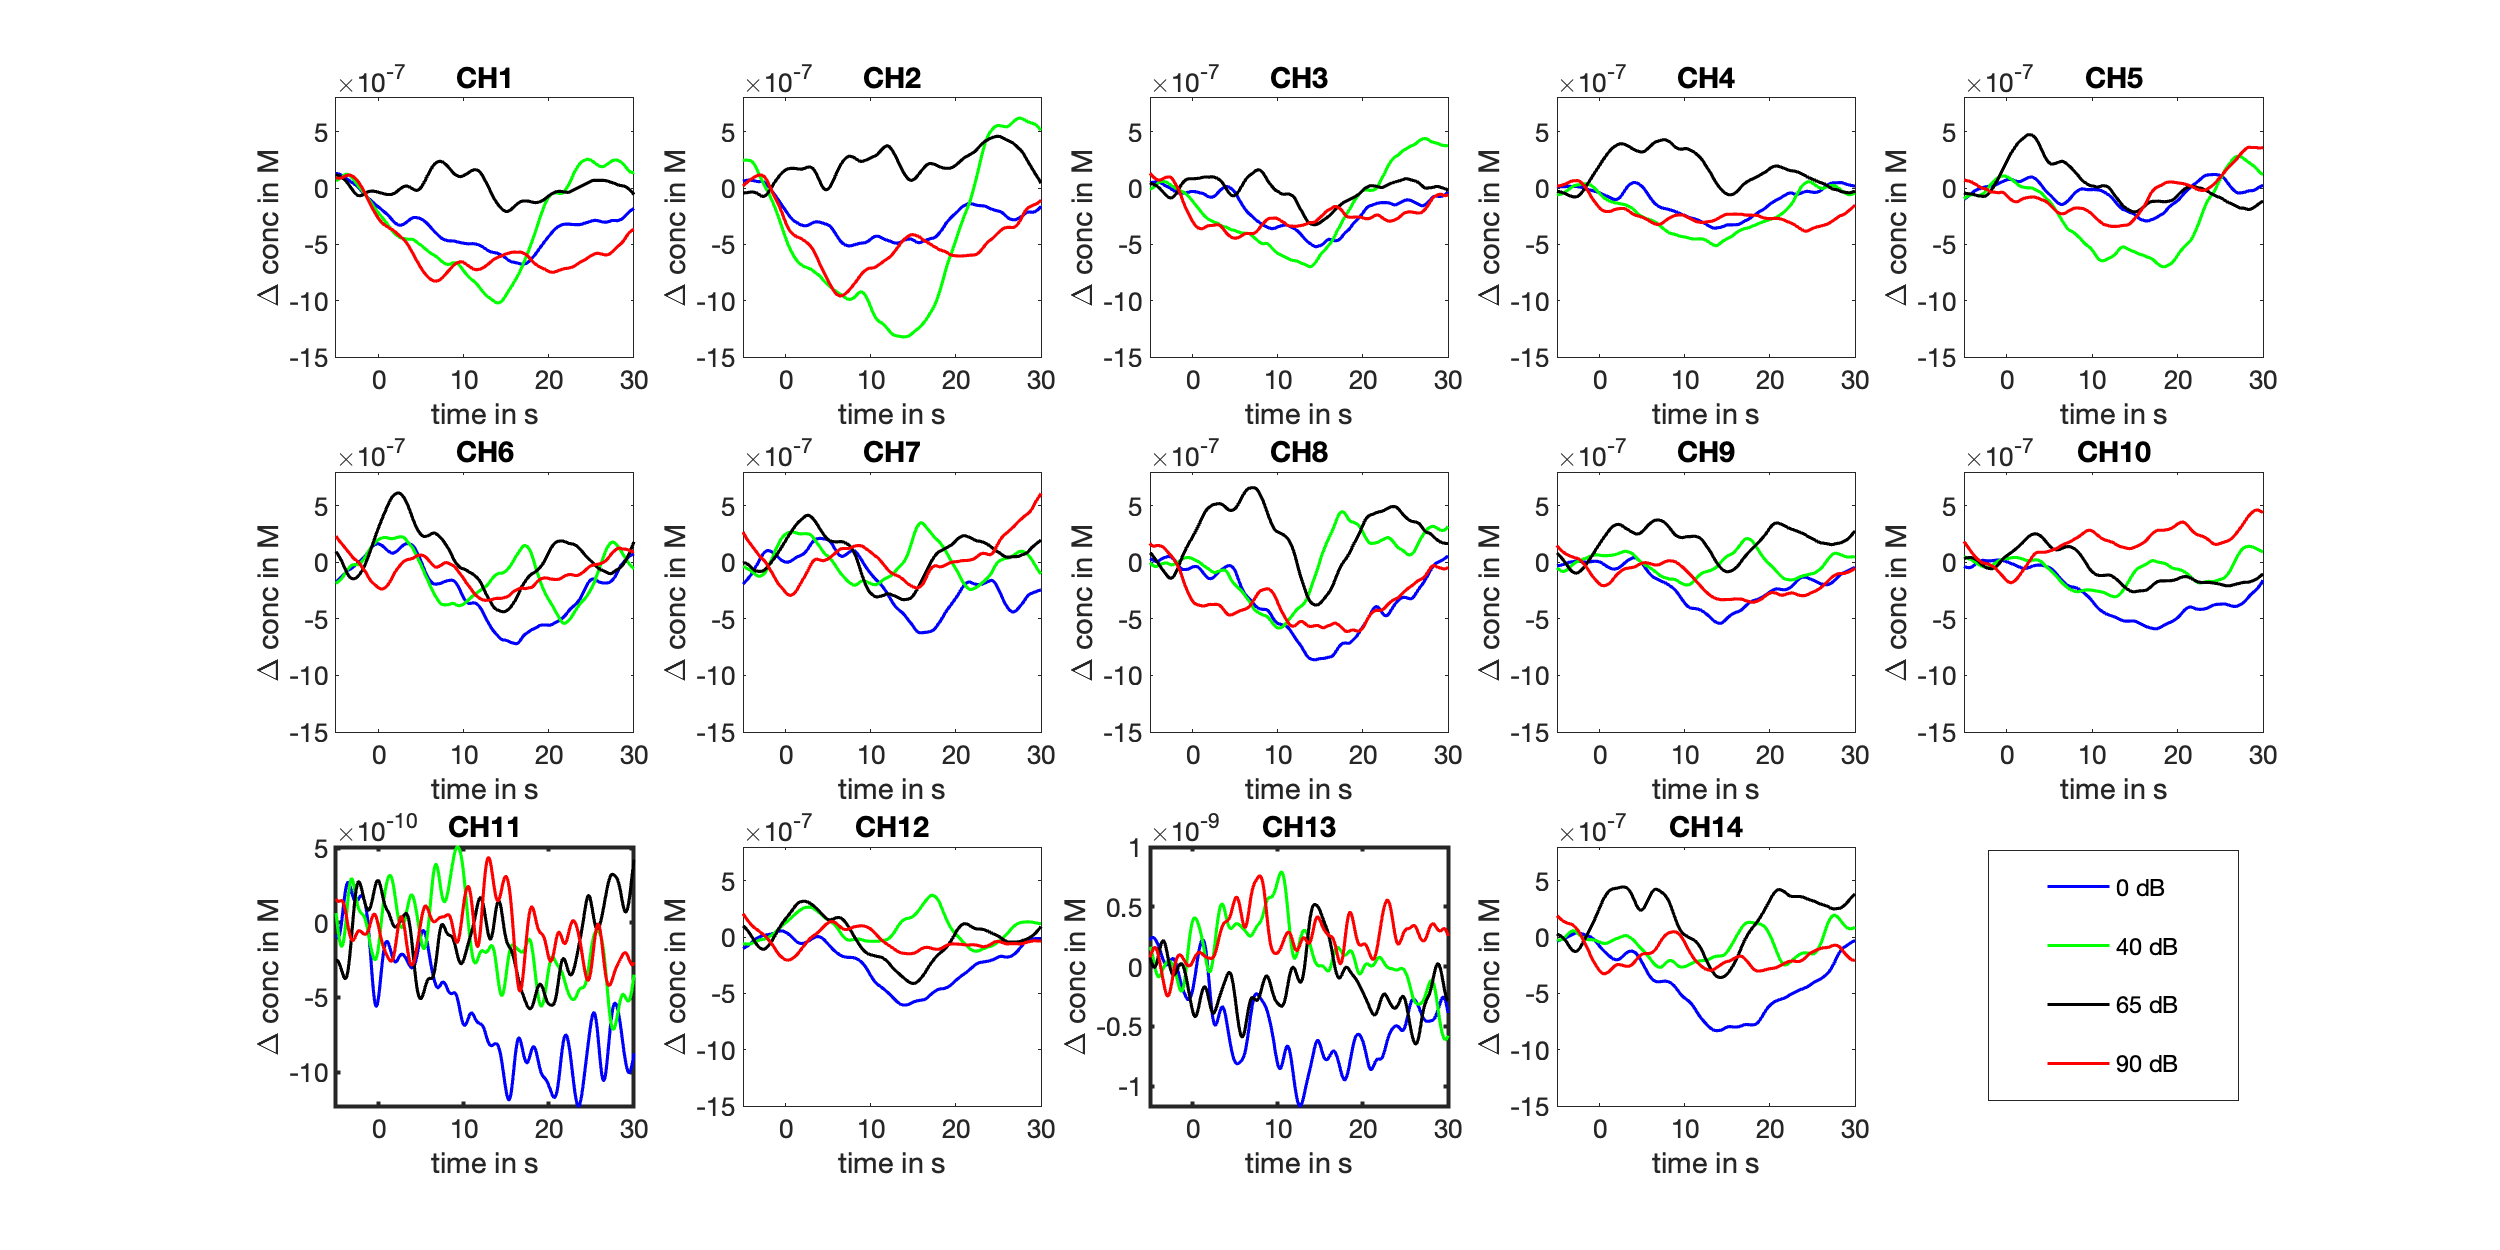
\includegraphics[scale=.4]{bilder/HbO_Mole/sub_luca2_s_HbO.png}
  \caption{Probe design in this research. Shown in AtlasViewer}
  \label{fig:somesignal}
\end{figure}

\begin{figure}[H]
  \centering
    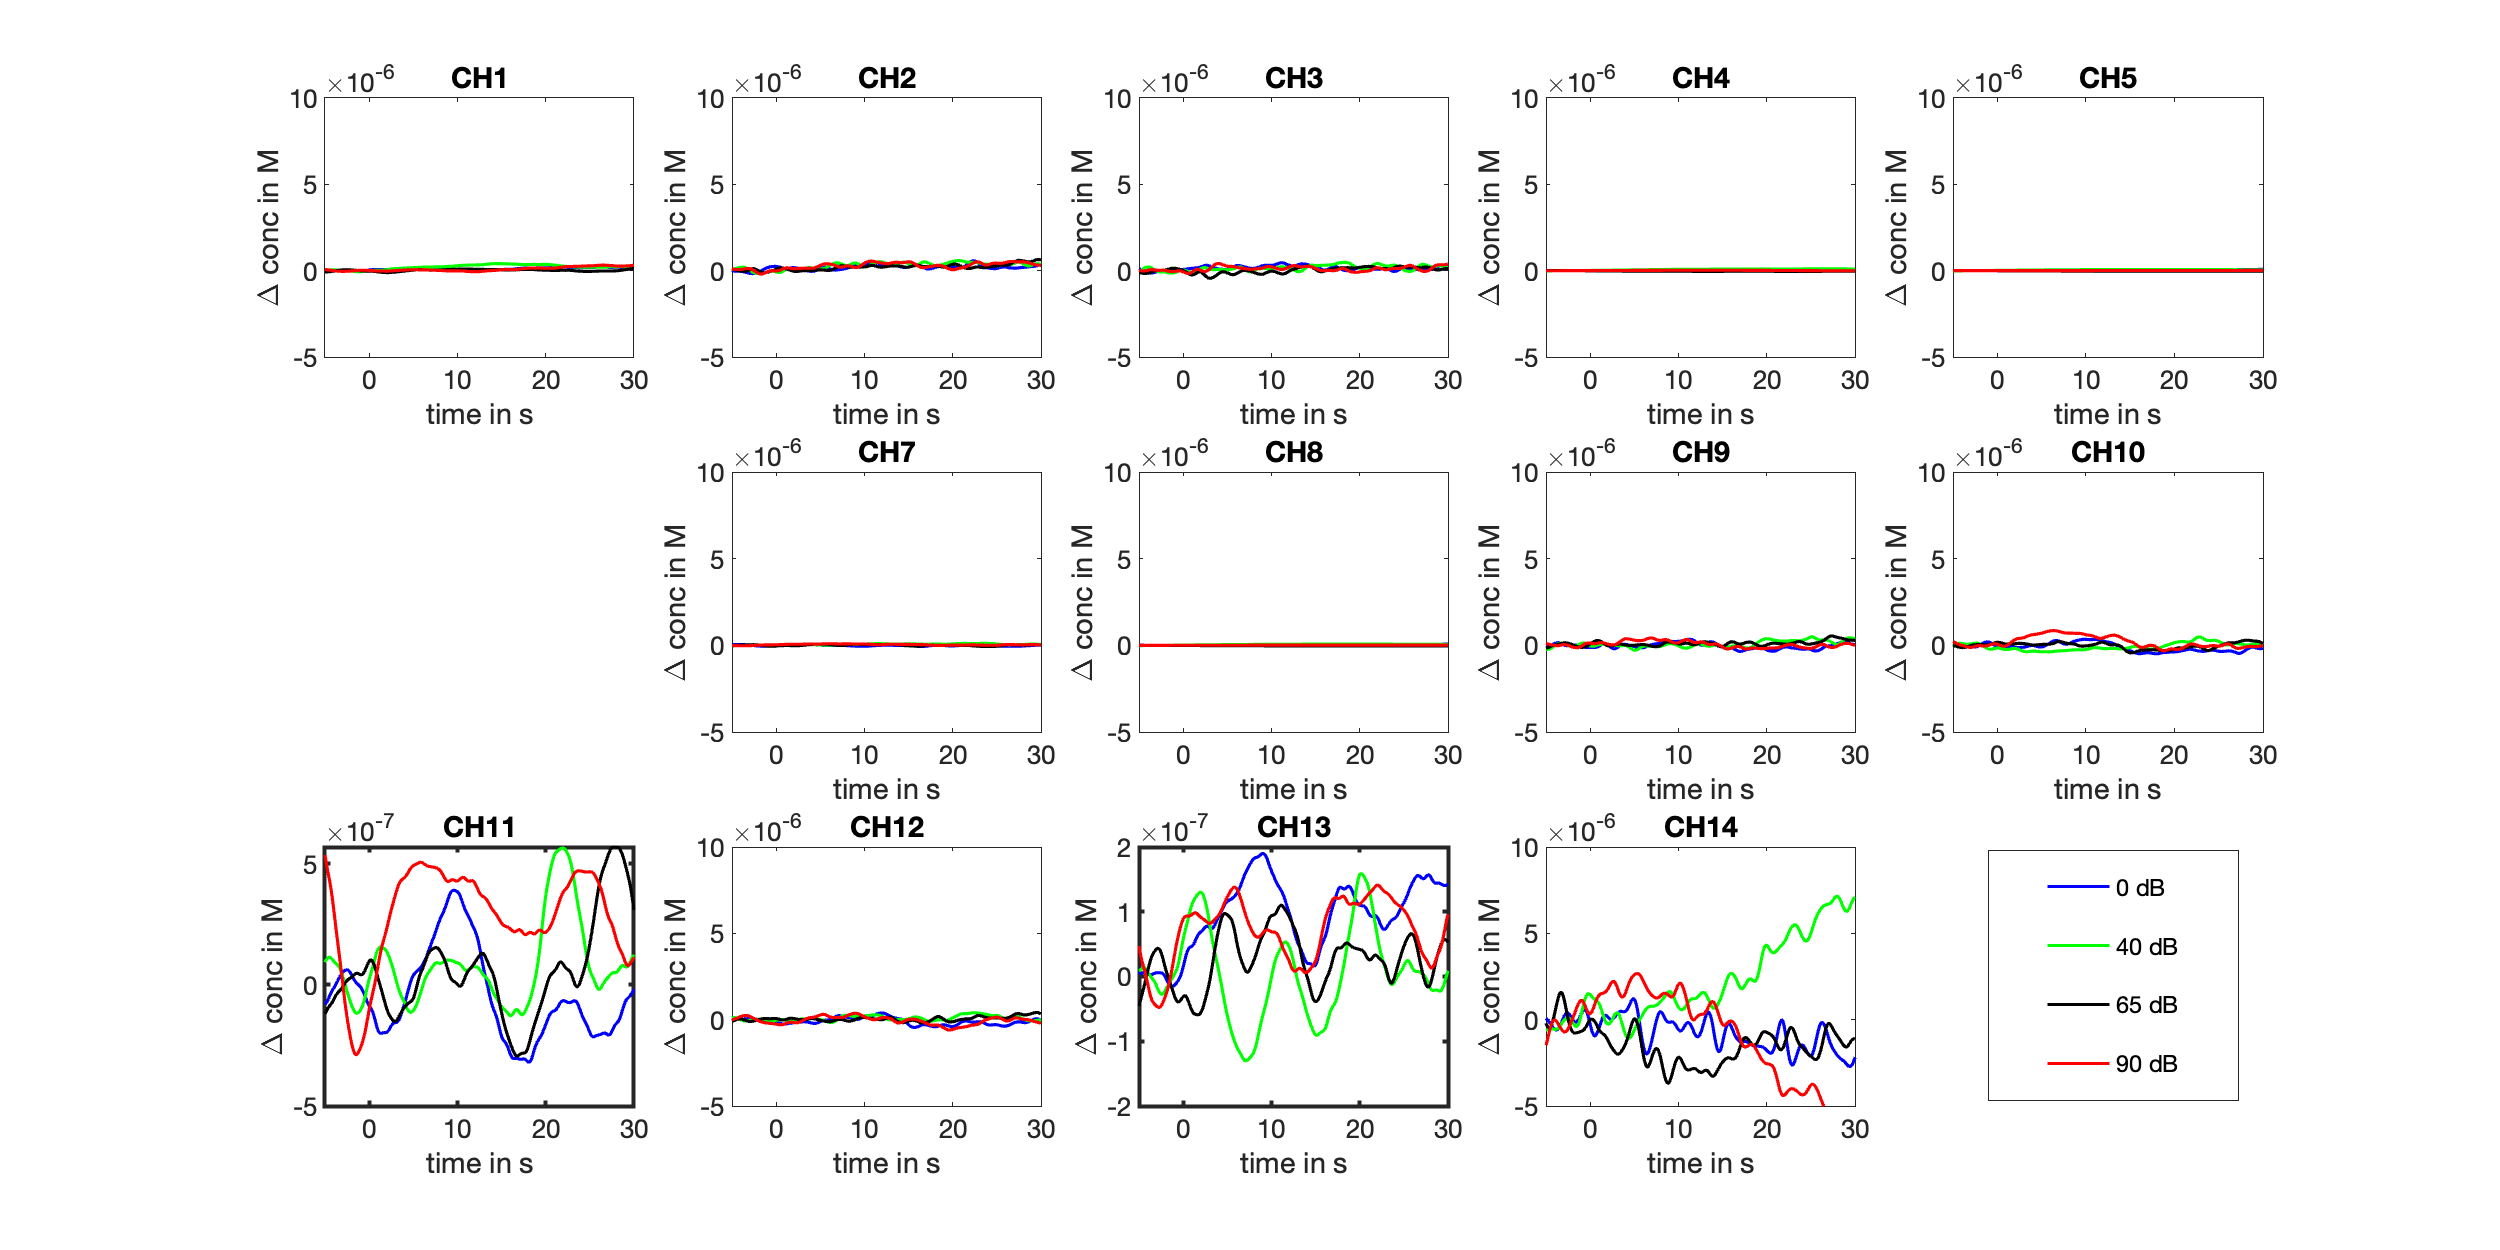
\includegraphics[scale=.4]{bilder/HbO_Mole/sub_lin_s_HbO.png}
  \caption{Probe design in this research. Shown in AtlasViewer}
  \label{fig:somesignal}
\end{figure}

\newpage

\section {Regional of Interest}

\begin{figure}[H]
  \centering
    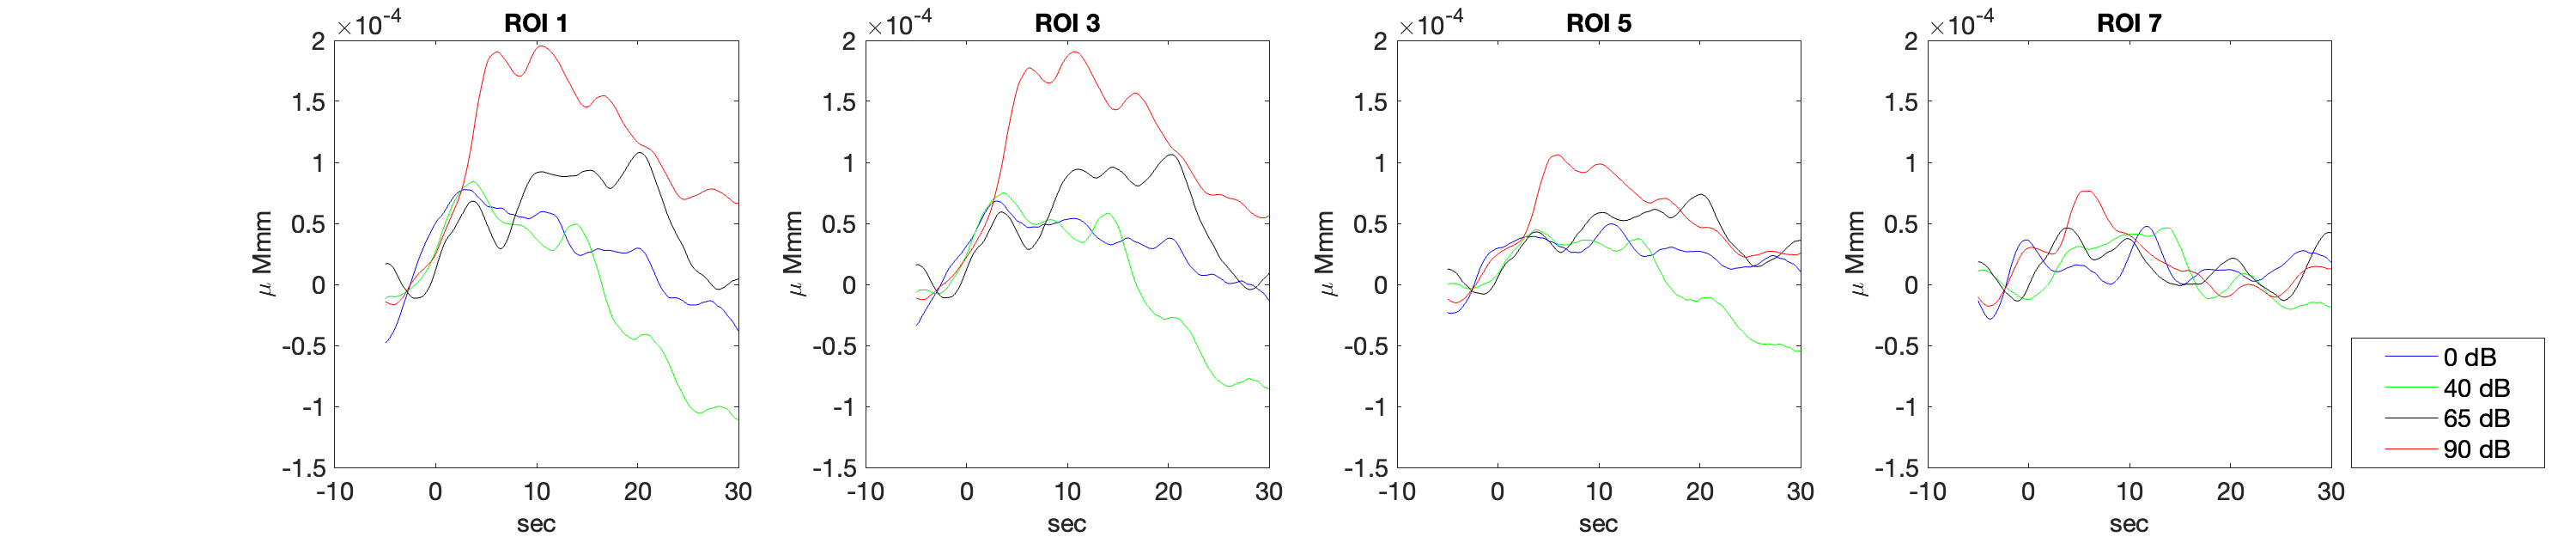
\includegraphics[scale=.3]{bilder/ROI/sub_jonas_s_HbO.png}
  \caption{Probe design in this research. Shown in AtlasViewer}
  \label{fig:somesignal}
\end{figure}

\begin{figure}[H]
  \centering
    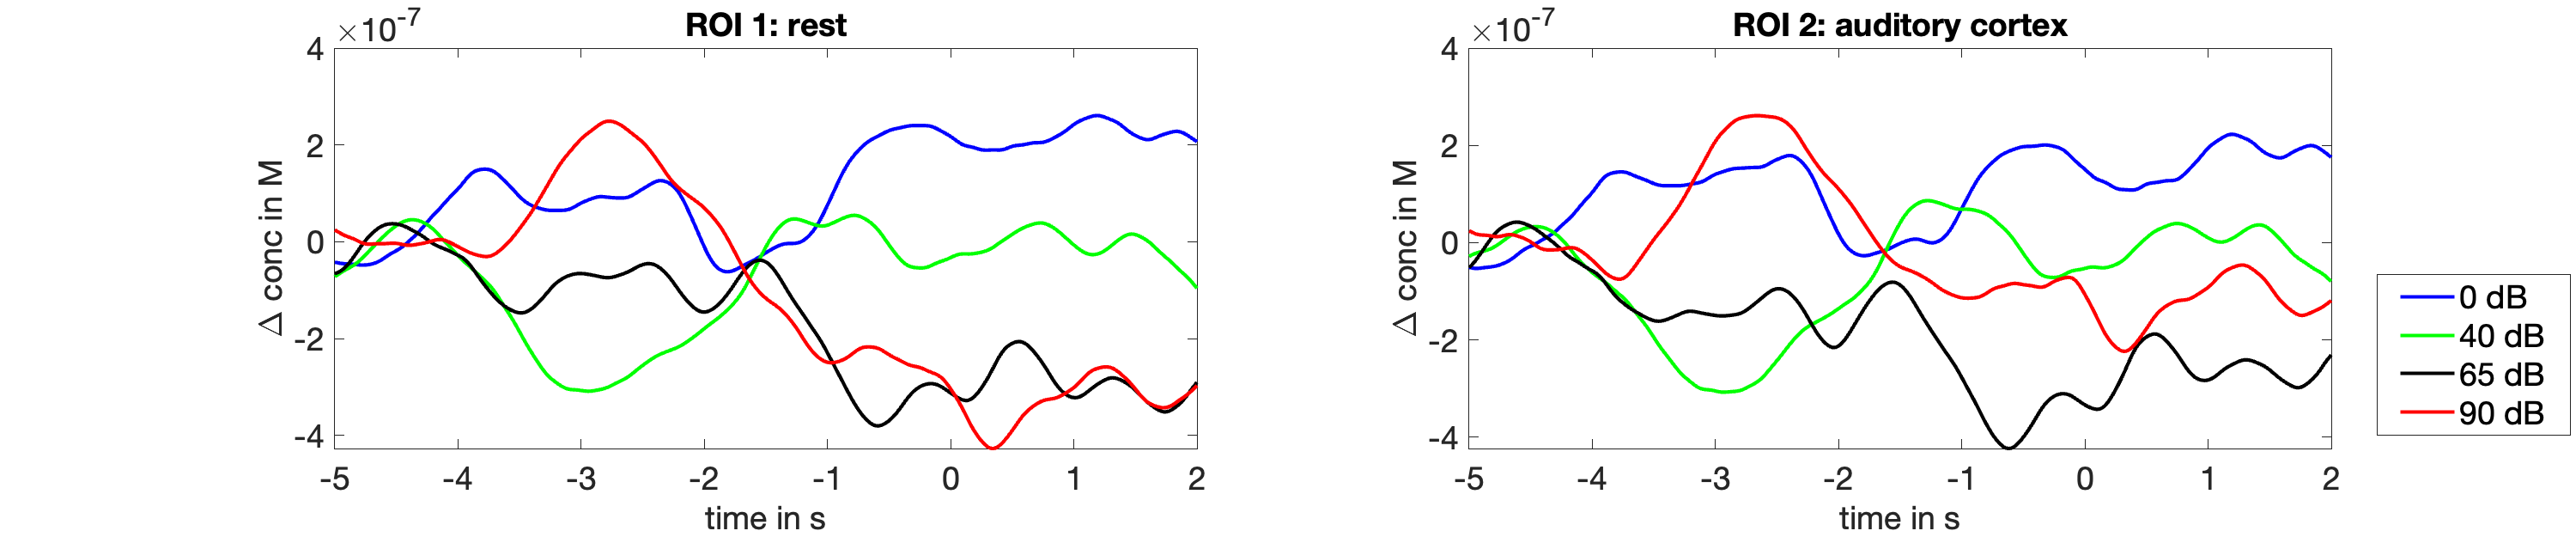
\includegraphics[scale=.3]{bilder/ROI/sub_lukas_s_HbO.png}
  \caption{Probe design in this research. Shown in AtlasViewer}
  \label{fig:somesignal}
\end{figure}



\begin{figure}[H]
  \centering
    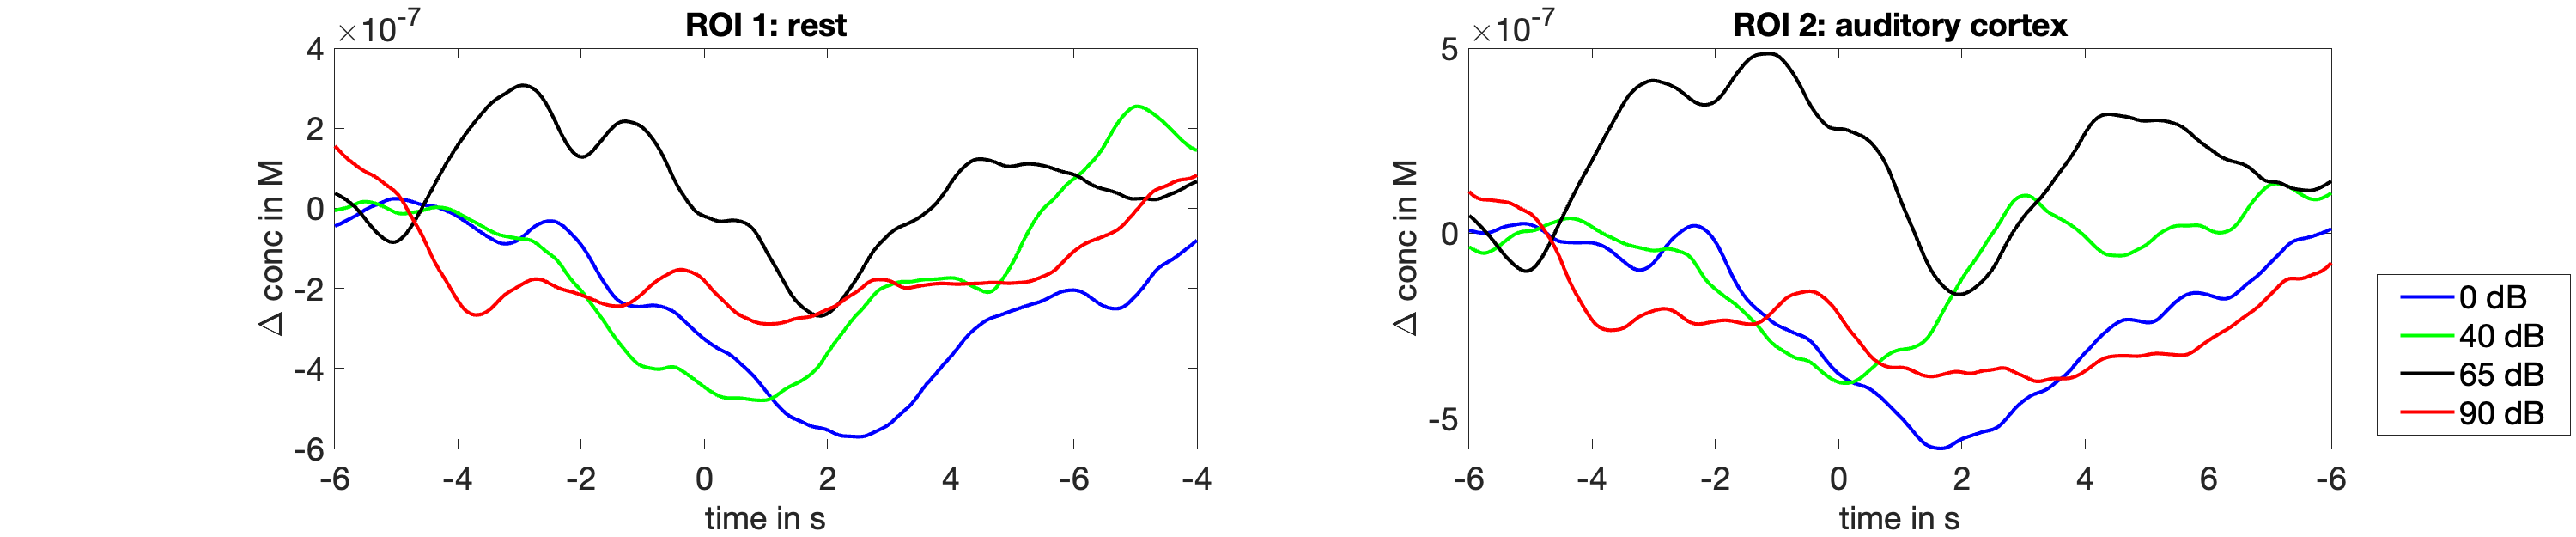
\includegraphics[scale=.3]{bilder/ROI/sub_luca2_s_HbO.png}
  \caption{Probe design in this research. Shown in AtlasViewer}
  \label{fig:somesignal}
\end{figure}


\begin{figure}[H]
  \centering
    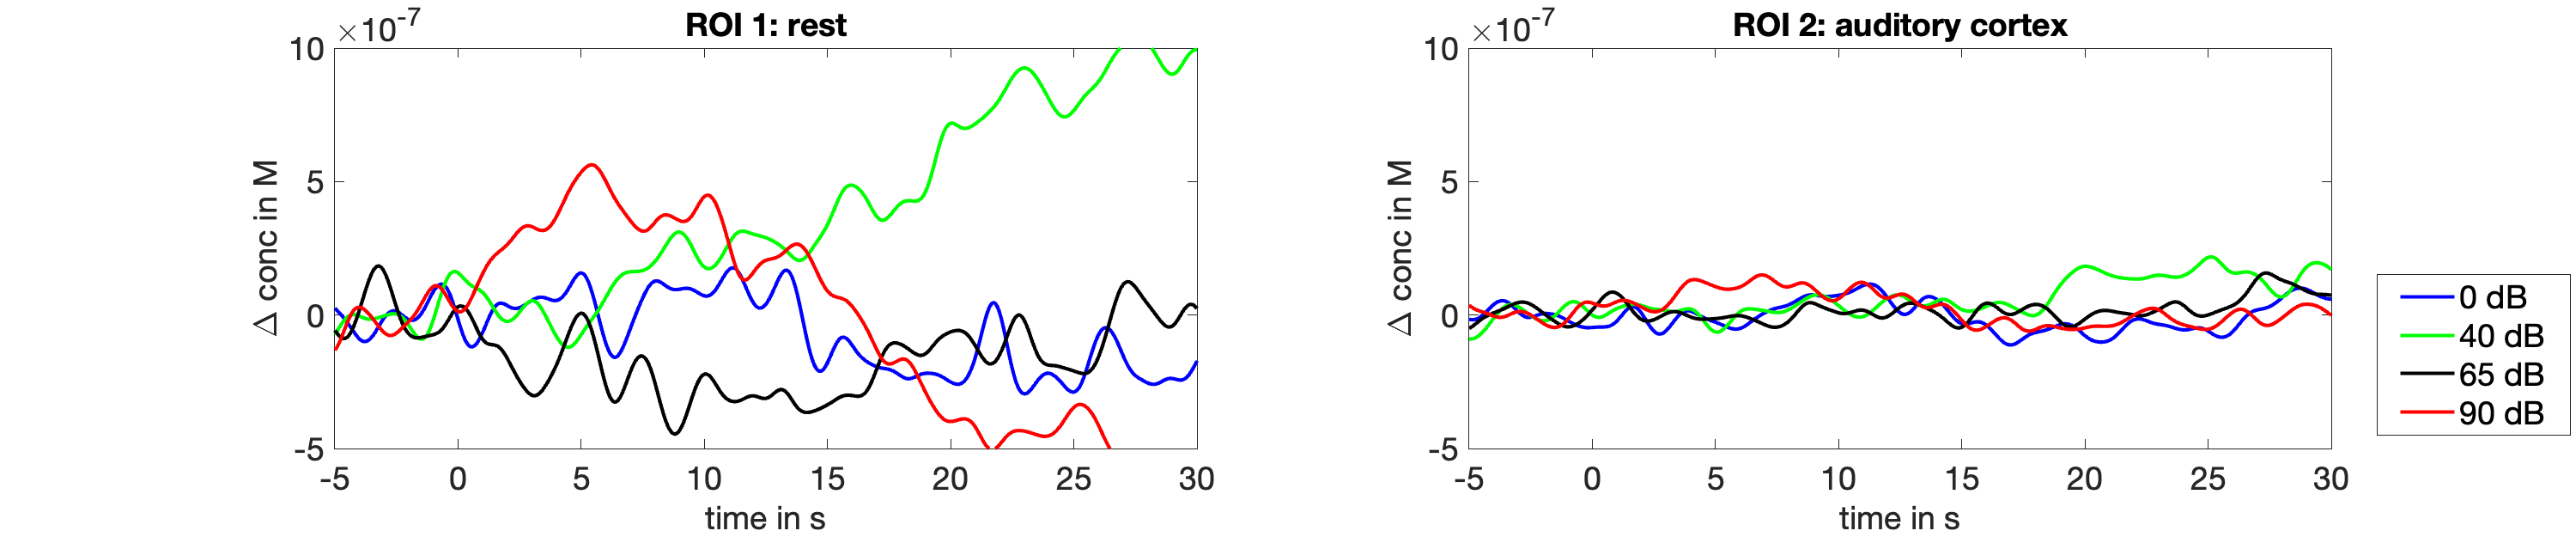
\includegraphics[scale=.3]{bilder/ROI/sub_lin_s_HbO.png}
  \caption{Probe design in this research. Shown in AtlasViewer}
  \label{fig:somesignal}
\end{figure}